\documentclass[12pt, letterpaper]{article}
\usepackage{xcolor}
\usepackage{parskip}
\usepackage{hyperref}
\usepackage{graphicx}
\usepackage{geometry}
\usepackage{setspace}
\usepackage{subcaption}
\usepackage{anyfontsize}
\usepackage{indentfirst}
\usepackage[utf8]{inputenc}
\usepackage[american]{babel}
\usepackage[babel]{csquotes}
\usepackage[notes,isbn=false,backend=biber]{biblatex-chicago}

\addbibresource{IA.bib}
\defbibheading{bibliography}{\section{Bibliography}}
\bibliography{IA}
\renewbibmacro*{cite:ibid}{\printtext[bibhyperref]{\bibstring[\mkibid]{ibidem}}}

\geometry{letterpaper, portrait, margin=1in}
\graphicspath{{./imgs/}}

\definecolor{url}{HTML}{4682B4}
\definecolor{cite}{HTML}{36648B}
\definecolor{link}{HTML}{344152}
\hypersetup{
  colorlinks=true,
  linkcolor=link,
  urlcolor=url,
  citecolor=cite,
}

\title{Media and its Effect on Aum Shinriky\=o}
\author{Simon Abrelat}
\date{May 2019}

\newcommand{\sorta}[1]{`#1'}
\newcommand{\poses}[1]{#1's}
\newcommand{\say}[1]{``#1''}
\newcommand{\Aum}[0]{Aum Shinriky\=o }

\begin{document}
%\large
\doublespace{}
\parindent=0.5in

{\fontsize{12}{14.4}
  {\singlespace
    \pagenumbering{gobble}
    \maketitle
    \begin{center}
    002129-0004 \\
    \vspace{4mm}
    IB History HL IA \\
    \vspace{4mm}
    Words: 2843 \\ % words
    \vspace{4mm}
    Candidate Number: \\
    \end{center}
  }
}	


\newpage
\tableofcontents
\pagenumbering{arabic}
\newpage

\section{Evaluation of Sources}
Aum Shinriky\=o is a doomsday cult that was based in Japan, which is primarily known for their Sarin gas
attacks on the Tokyo subway system. It thrived on the spiritual void in the \poses{80} and  \poses{90},
and used popular culture for their recruitment. A cult lives and breathes on its members and perception,
just think about the siege of the Branch Divisions at Waco, Texas, the mass murder suicides of the Order of
the Solar Temple, and Jonestown. Cults get violent when there practices get brought to the light. So, to
what extent can the popularity and the downfall of Aum Shinriky\=o be attributed to the media?

\subsection{\citetitle{watanabe_reactions_1997}}
\say{Reactions to the Aum Affair: The Rise of the \sorta{Anti-Cult} Movement in Japan.} is an essay is based
on a paper presented at the annual meeting of American Academy of Religion in 1996
\footcite{watanabe_reactions_1997}. It
was published in the 21\textsuperscript{st} .Volume of the annual Bulletin for the Nanzan Institute for
Religion and Culture. This separates the \say{Aum Affair}, the time between being approved as a religious
institution and the gas attacks, into four different periods.Th  first period was as it budded into its
current form, the second is the beginning of negative press, the third is a time were \say{intellectuals 
  \footcite[33]{watanabe_reactions_1997} reevaluated} Aum Shinriky\=o, and finally, the forth is the gas attacks to there downfall. This resource is valuable because of how it tracks the criticism of the cult and
they way Aum Shinriky\=o responded. Their typical response being murder. This paper showed the causal
relationship between the level of criticism and violence which led to their downfall. The main issue with
this paper is that it does not explain the media practices used by Aum Shinriky\=o, the cultural context, or
what made them gain so much power. The main purpose of  this paper was to show how new religious or spiritual
movements can clash with culture at large for an academic conference.

\subsection{\citetitle{noauthor_cult_nodate}}

This source is a WIRED article in 1996 \footcite{noauthor_cult_nodate}. This was one year after the infamous gas attack. The main purpose 
the article is to illustrate the sort of people that would get sucked into this cult, the Otaku. An otaku
is a nerd that immerses themself in anime, manga, and Japanese cartoons and popular culture to the point of
becoming detached with reality and in generally a derogatory term. The stereotype is also focused around 
nerdy men. The article reflects the mainstream perception of the cult members being lost, young, 
otaku men. It gives a few second hand accounts from former cult members and highlights examples of 
prominent scientists that got taken in. The limitations are that there are no examples of their recruitment
materials that cater to otaku, and how they continue with the stereotype of demeaning otaku. They mention
the societal issues, but attributed most of the recruitment to violent anime and science fiction stories.
This article also shows the attitude toward the cult at time when they were at their most well-known. 

\section{Introduction To Aum}
Aum Shinriky\=o is a Japanese cult that started operating in 1987 and was granted status as an Religious
Cooperation in 1989 by the Tokyo Metropolitan Government. The cult was started by Asahara Shoko, birth-name
Chizuo Matsumoto, who is believed to subject to \textit{pseudologia phantastica}
\footcite[5]{olson_aum_1999}, otherwise known as pathological lying. He later developed sever
incarceration psychosis \footcite[6]{olson_aum_1999} over the course of his trials before getting
the death penalty. The disconnection between reality and story, and sometimes violent actions taken by
pathological liars to maintain their story, point to why media caused such violence by Asahara and his
followers. Aum is an outstretch of a larger \sorta{New Religion} wave in Japan, and was, in many
ways, an offshoot of Agonshu \footcite[82,83]{watanabe_religion_1998}. During his time with Agonshu, he
started to mix Buddhism and Yoga. Yoga, in the religious sense, being one of the six orthodox schools of 
Hinduism. With his connection to Yoga, he chose Shiva, "The Destroyer", as his main deity. For his own Buddhist
practice, he went to Tantra Vajrayana which is a Tibetan esoteric Buddhist sect. Asahara took the basic ideas from
Agonshu and synthesized them with other religious practices to create a system that applies to a broader 
range of people. He mixed disparate ideas from generally peaceful religious practices to form a foundation 
for violence and control.

\subsection{Beliefs}
The beliefs of Aum are a complex mix of Buddhism, Yoga, and aspects of Christianity, more specifically the
idea of a messianic leader \footcite[1144]{metraux_religious_1995}. For Buddhism, the Vajrayana tradition is 
a subcategory of the Mahayana sutras and the borrowed the idea of Ten Realms (jikkai) from the Lotus sutra.
When someone is reincarnated based on their karma (level of morality as determined by their actions and
thoughts), they could return to any of the six rebirth realms:  Hell, Hungry Ghosts (pretas), Beasts, Titans
(Asuras), and Humans \footcite[83]{watanabe_religion_1998}. Aum also uses the idea of the Three Ages 
of Buddhism: sh\=ob\=o, z\=oh\=o, and mapp\=o. Sh\=ob\=o is the period were Dharma (behavior in accordance
to the cosmic law) is at its highest, and Mapp\=o, the Degenerate age, is were Dharma has all but 
disappeared. Asahara claimed that he had awoken his Kundalini (serpent power) which is located in the lower
spine. It is seen as the origin of supernatural and the energy source for spiritual. Later, Asahara co-opted
the idea of Poa, or phowa, from more violent esoteric Buddhist sects. Poa is a Tibetan term for the 
transference of consciousness, or, in other words, death. A skilled enough practitioner could transfer a 
consciousness to a higher realm. Asahara weaponized this concept to make killing at his order virtuous.

One of \poses{Aum} central beliefs was that the world was in such a state of moral decline that a beast is 
more likely to reincarnate to a higher realm than a human. Asahara he had a revelation through Shiva and has
reached the tenth realm of buddhahood. Shiva had told him that he would bring in a age of sh\=ob\=o, and
usher in Shambhala. Poa then purifies the social Dharma from the state during Mapp\=o, raising the 
Dharma of the new kingdom and raising a human from the realm of hell. The goal of Aum was to cause the 
Harumagedon, or Armageddon, to cause the second period of Sh\=ob\=o.

\section{Media}
\subsection{Recruitment}
Since Aum preaches about societal decay, the people influenced by the cult would, in general, be the 
outcasts. In Japanese culture, the socially inept and isolated are the otaku. If a person is so deeply interested or
addicted to something to the point they are dysfunctional, then they are an Otaku. There are train Otaku or
art otaku, but the colloquial use of otaku is in reference to anime, Japanese cartoons.  Some of these otaku
where taken out of top scientific university. Those being the type of anti-social nerds that thrive in
academic or scientific studies, but fail to live a complete life beyond that. Appealing to otaku culture and
outcasts as well as giving people a broader purpose and superiority were some of the draws for the cult. Aum
and their image of Harumagedon parallel the post-apocalyptic anime of \textit{Space Battleship Yamato} and
\textit{Akira} and the idea of battle between a smaller righteous force prevailing is similar to
\textit{Mobile Suit Gundam} \footcite{macwilliams_japanese_2008}. Given \poses{Asahara} blurring of reality and fiction, he drew parallels between these franchises and Aum. 

Beyond the over-sensationalized news articles about the dangers of Otaku 
\footcite{noauthor_mike_nodate}\textsuperscript{,}
\footcite{noauthor_cult_nodate}, the disillusionment of the youth can be somewhat attributed the culture in
post-WW2 Japan and the development of postmodernism in Japan. With the addition of Western culture, 
capitalism and industrialization, the centuries old Japanese culture and narratives started to morph. Hiroki
Azuma, a Japanese philosopher and cultural critic, states that the Anime that Aum takes inspiration from 
where from \sorta{The Period of Fictions}. The Period of Fictions was when people were still looking for the
old stories to make it through modern life, and Aum comes it to provide similar catharsis for its followers.
It would then make sense that Aum would borrow aspects from these franchises or cater to similar audiences.

% Hiroki Azuma is a japanese philosopher that separates post-war Japan into 3 periods: The
% Period of Ideals, The Period of Fictions, and The Period of Animals. The Period of Ideals is the
% pre-postmodern 
% period where the grand cultural narratives are still intact. The Period of Fictions is the early postmodern
% period where the grand narrative is dissolving, but people still cling to their security. This is the point
% were the grand narrative started to fracture into smaller meta-narratives, this is also the period where
% \textit{Space Battleship Yamato}, \textit{Akira}, and \textit{Mobile Suit Gundam} were made. This period
% started after the failed communist revolution \footcite[12]{kane_repackaging_2016}. The Period of Animals,
% for
% Azuma, begins after the 1995 Sarin Gas attack, and represents the total decline of the grand narrative and
% people have moved on instead gaining meaning by choosing their story from the cultural \sorta{database}.
% Instead of beckoning in the new era of Sh\=ob\=o, Aum marks the turning point to total postmodernizaiton in
% Japan. The other anime which has aspects similar to Aum and also straddles the periods of Fictions and
% Animals is \textit{Neon Genesis Evangelin}. 

There are several specific examples of Aum recruitment material, but a new offshoot, Aleph, has rights to all
of it. Aleph somewhat restricts the old material and send copyright strikes against illegal uploads. Despite
that, there are some open Aum Anime \footcite{noauthor_aum_nodate}\textsuperscript{,} \footcite{noauthor_aum_nodate-1}.

\begin{figure}[h]
  \caption{Aum Manga}
  \label{fig:aumManga1}
  \centering
  \begin{subfigure}[b]{.4\linewidth}
    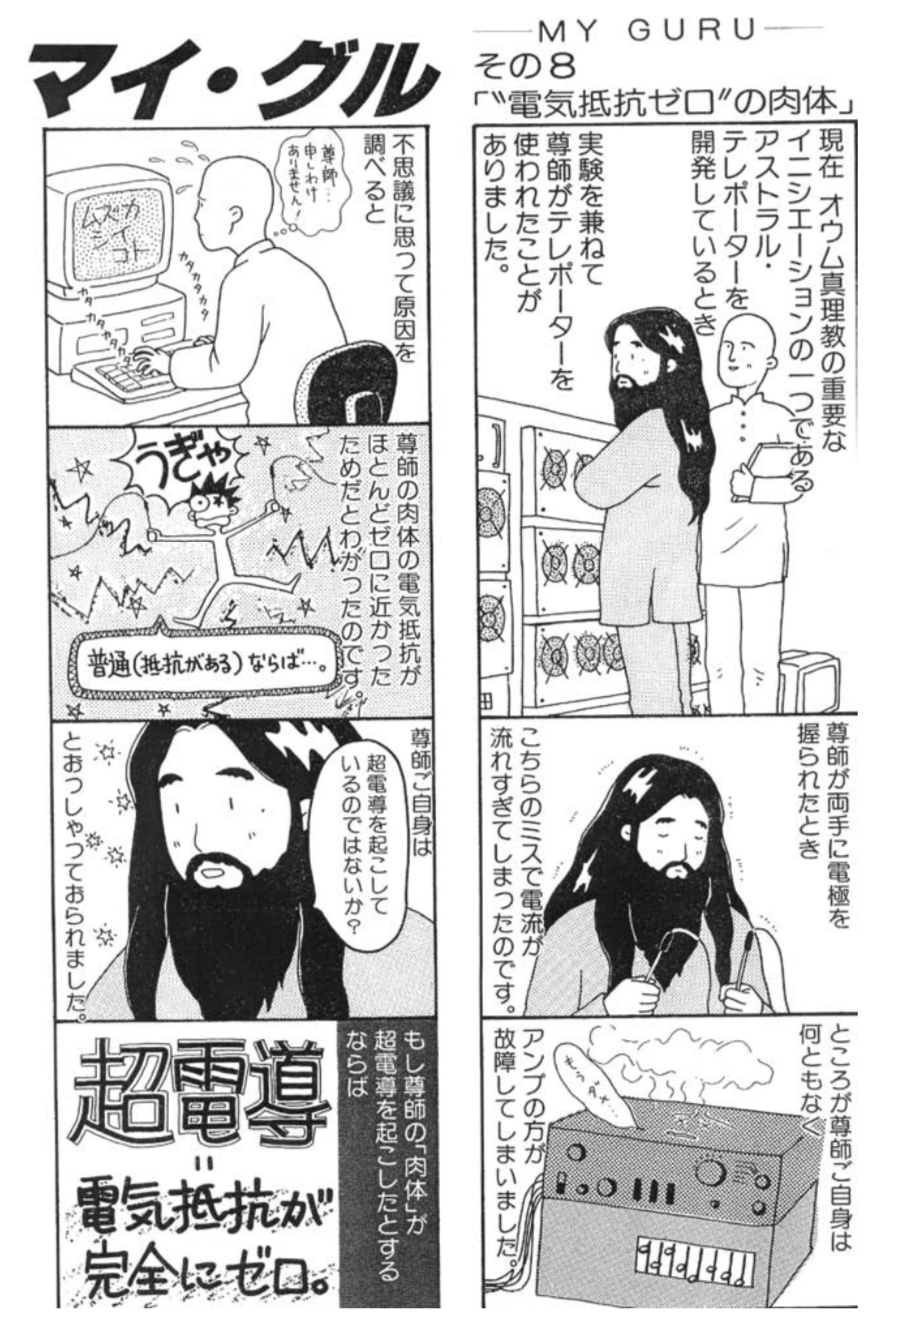
\includegraphics[width=\linewidth]{myGuru.png}
    \caption{My Guru}
  \end{subfigure}
  \begin{subfigure}[b]{.4\linewidth}
    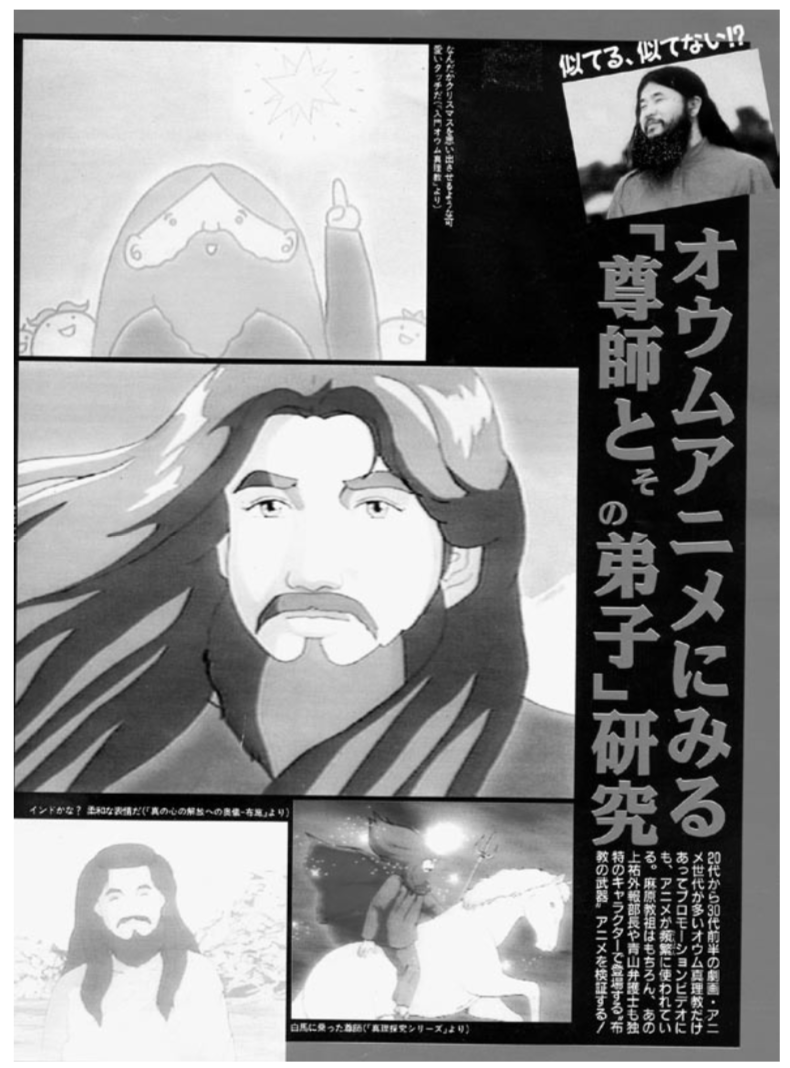
\includegraphics[width=\linewidth]{flyer.png}
    \caption{Recruitment Flyer}
  \end{subfigure}
\end{figure}

\begin{figure}[h]
  \caption{Harumagedon}
  \label{fig:harumagedon}
  \centering
  \begin{subfigure}[b]{.9\linewidth}
    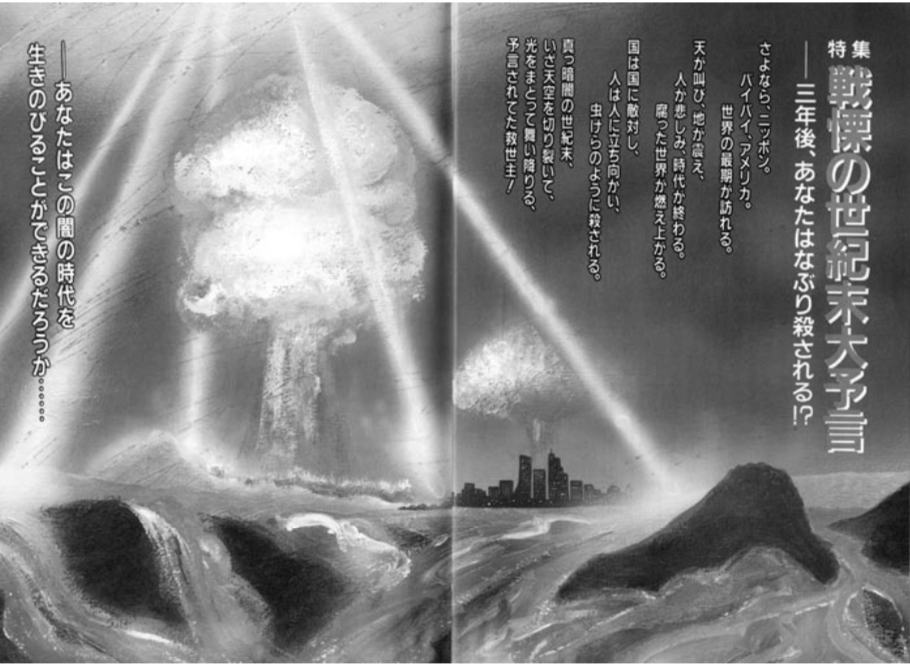
\includegraphics[width=\linewidth]{harumagedon.png}
  \end{subfigure}
\end{figure}

Figure \ref{fig:harumagedon} and \ref{fig:aumManga1} are examples of Aum publications in three different
styles of Manga. These types of materials emphasize \poses{Asahara} powers.For example, Figure
\ref{fig:aumManga1}a is a manga called My Guru where they test his body for resistance, and his
body ,strangely ,has none. The lack of resistance shows his attunement with energy. In \citetitle{noauthor_aum_nodate} Asahara is shown connecting to others spiritually,
astral traveling, and levitating with a sideshow of pictures of Asahara at the end.
\citetitle{noauthor_aum_nodate-1} is a story of two naked people akin to Adam and Eve interspersed with
strange images of cities and fields of grain. The video is in Japanese without subtitles, so without
translation, the most that can be draw from that video is the clear biblical allusion.

\subsection{Decline}
There first major media exposure was in the \textit{Sunday Mainichi} through a seven article series called \say{The Insanity of Aum
  Shinriky\=o} in September of 1989 \footcite[35]{watanabe_reactions_1997}. This media attention had started
just after they got their religious cooperation distinction. On October  2\textsuperscript{nd}, they
published a series of interviews with six families that claimed that Aum had stolen their kid from them, not
kidnapped but brainwashed \footcite[184]{hardacre_aum_2007}. After these stories came out, the families of
Aum monks started to band together into the Association of Aum Shinriky\=o Victims under the lawyer Sakamoto
Tsutsum. Sakamoto and his family disappeared on November 4\textsuperscript{th} and assumed dead. Later, in
September 1995, It was confirmed they were killed by Aum
followers and their bodies were recovered. Beyond being the groups first killings, this event was important
since it was the first use of Poa justified killings, a hallmark of Aum 
\footcite[89]{watanabe_religion_1998}. Sakamoto was opposing \poses{Aum} expansion and decreasing Dharma by
stopping them; therefore, using Poa to kill him would be saving him and increasing Dharma getting everyone
closer to Sh\=ob\=o. \poses{Aum} goals of expansion came in buying large plots of land Kamikuishiki-mura in
1990 and entering the general election under \sorta{the Supreme Truth Part}\footcite[187]{hardacre_aum_2007}.
All of these attempts were stopped by locals of The Association of Aum Shinriky\=o Victims. All of their
candidates failed and the legal battles for the land sewed a greater distrust of the Japanese government.

% To add insult to injury, they bought large plots of land in small villages around Kamikuishiki-mura in 1990. Similar to other communes like Rajneeshpuram for Osho, the locals were unhappy with these communes and large communities suddenly converging on their towns.The Association of Aum Shinriky\=o Victims also came in and helped the locals voice anti-Aum sentiments. Another aspect of them bursting onto the scene was their attempt to get elected \footcite[187]{hardacre_aum_2007}. In February 1990, Asahara and twenty four other leaders inside Aum entered the general election under the Supreme Truth Party created by Aum for this purpose, and all of their candidates failed. This sparked even greater distrust of the Japanese government. 

There were some anti-Aum publications, but, as a
whole, they were receiving praise from religious scholars such as Shimada Hiromi and Nakazawa Shin’ichi
\footcite[38]{watanabe_reactions_1997}. Aum also had a public debate with K\=ofuku no Kagaku (The Science of
Happiness), another new religion group, on \say{Asa made nama terebi} (Live until Morning) which aired at
midnight September 28, 1991. During the debate, Aum appeared to show a deeper knowledge of Buddhism than
K\=ofuku no Kagaku, so they, subsequently, won. During this time, the biggest anti-Aum publications were done
by Egawa Sh\=oko, and some of her essays
became the seminal papers on this area publishing in weekly journals. In general, the positive TV appearances
and positive reviews outweighed the negative articles and this was a period where the media about Aum was
generally positive. Religious and Television personalities such as Shimada Hiromi, Nakazawa Shini'chi, and
Takeshi Kitano were warm to Aum and liked their public ideas. Even Yashimoto Takaati, a prominent philosopher
and public intellectual, give a favorable review to \poses{Asahara} writings. While hidden from the public,
Asahara had a limited number of his disciples to begin assembly of AK-47 machine guns and begin working on
the developing different nerve gas agents \footcite[91,92]{watanabe_religion_1998}.

In 1993, they successfully synthesized Sarin, and, by 1994, had
produced thirty liters of it. On June 27\textsuperscript{th} 1994 they did a smaller Sarin release in
Matsumoto killing seven people and injuring 144. This attack was to kill the judges who were providing over a
case in relation to \poses{Aum} Matsumoto branch office. None of the judges were killed, but they were 
wounded and the case was left dormant for months. The Japanese authorities did not know the perpetrators,
but, on January 1\textsuperscript{st} an article documenting new was published by Yomiuri Shimbun stating 
that some residue of the Sarin was found near an Aum facility in Kamikuishiki-mura, Satian 7. On February
28\textsuperscript{th} Kariya Kiyoshi was abducted by the group after offering a hiding place and way out of
the cult to his wealthy sister. For this, the cult forced a confession from him, the hiding place of his
sister, and, heavily drugged, killed him. The incident Kiyoshi was again a time where anyone obstructing Aum
would have Poa used against them. This is the first investigation done on Aum as an organization by
the police. The pressure on Aum from the authorities and civilian organizations as well as the increasing
production of chemical weapons meant that a larger incident was inevitable. In the beginning of March, Aum
followers started to hand out fliers for \poses{Asahara} new book \textit{Disaster is Approaching the Land 
  of the Rising Sun}. In the book he supposedly foretold the Hanshin Earthquake and talked about another
disaster to befall Japan. On March 20\textsuperscript{th} 1995, Aum Shinriky\=o sprayed Sarin gas in a
coordinated attack on 15 Tokyo train stations. The largest attack being on the Hbiya line involving between
300-400 victims \footcite[513]{olson_aum_1999}. In total 12 people were killed and 3,796 where injured in the
largest modern terrorist attack on Japanese soil.

\section{Conclusion}
% Asahara was a master manipulator. His possible mental instability, as manifested in pseudologia.phantastica
% and eventually psychosis, allowed him to blur the lines between religion and pop culture. In his inability to
% adequately separate story and reality, he and his philosophies embody the breakdown on traditional narratives
% but clinging on to a greater purpose. In this "Era of Fictions", media played a large role in giving people
% value and purpose since it was a form of escapism. This escapism gave Aum power since they used the people
% seeking a way out to gain power and influence, but in that system of fast growth, they blew up. An upwell of
% anti-Aum articles and media cemented their already paranoid and anti-social beliefs and meant that the
% already unhinged \poses{leader} lies were falling apart.

The story of Aum is that of violence and manipulation. They used a mixture of religions to gain wide spread
appeal and use the media to target the downtrodden and \sorta{give them a voice}. Aum always had vocal
antagonists, but eventually they gained enough power and exposure to become more publicly respected. With the
mix between esoteric Buddhism and Hinduism, they justified all of their actions and only increased their
fanaticism. The ability which Asahara had to tap into societal issues and weaponized them was impressive. The
ability to twist fantasy and relate to connect anime and cultural narratives to religious action is
unparalleled. Because of their ability to connect to people, Aum was able to gain popularity and become a
unrivaled terroristic force in Japan.

\section{Reflection}
Like many emotionally-charged, historical events and movements, the importance of Aum Shinriky\=o is overstated and
people quick to criticism. There is a strong conversation about the media's portrayal of otaku in these 
events and where they were used for a scapegoat for broader cultural issues. The problem is that these
conversations are mainly on online message boards, so not conducive for academic decision and, if it were,
beyond the scope of this investigation. One of the complications historians run into was in what people chose to omit
or neglect to mention. For example, in the Decline section, there was \citetitle{watanabe_reactions_1997} 
that had a nice framework for how media affected Aum and their paranoia, but it did not say anything about
police investigations. In fact, to pull together the events before the Tokyo Subway Attacks I had to
synthesize information from another of \poses{\citeauthor{watanabe_reactions_1997}}
works\footcite{watanabe_reactions_1997}\textsuperscript{,}\footcite{watanabe_religion_1998}. Each article is
highly specialized given the size and implications of this topic so it requires combining multiple sources to
approach a timeline of important stressing events. People would also reference the beliefs of Aum, but
tracking down how specific elements of culture and religion interact was also difficult. With the exception
of \citetitle{watanabe_religion_1998}, the most detail papers talk about their beliefs is yoga and Poa. This
project is basically impossible to explain in its fullest since I have not documented the affects on Asahara
himself or go into specific detail on their brainwashing techniques and cult indoctrination required to plain
recruitment and operation. There was also a wealth of new religions popping up in Japan in this time, so
further exploration into the landscape of religion and spiritualism in \poses{1980} Japan would help this
essay. Any topic worth covering has a ridiculous amount of detail so it is a constant
challenge to battle the specific research used to make a given point, and make sure intellectual integrity is
maintained. Although those topics would be useful, it would be impossible to fit all of the information to
adequately cover these issues in this paper.
\newpage
\printbibliography{}
\newpage
\section*{Appendix}
\listoffigures{}
\end{document}
